%!TEX root = ../../thesis.tex
\section{App Packaging}

For better and faster access on mobile phones, XBMCMagic is packaged as mobile application using the Phonegap\footnote{\url{http://phonegap.com/}, last-checked on 23/04/2014} build chain. Phonegap provides a way of creating so-called hybrid mobile applications. It takes the source web files of the application and wraps them into a simple mobile application which serves the web content through a native WebView on the device. This allows developers to create mobile applications from web applications. 

\begin{figure}[htb]
  \centerline{
    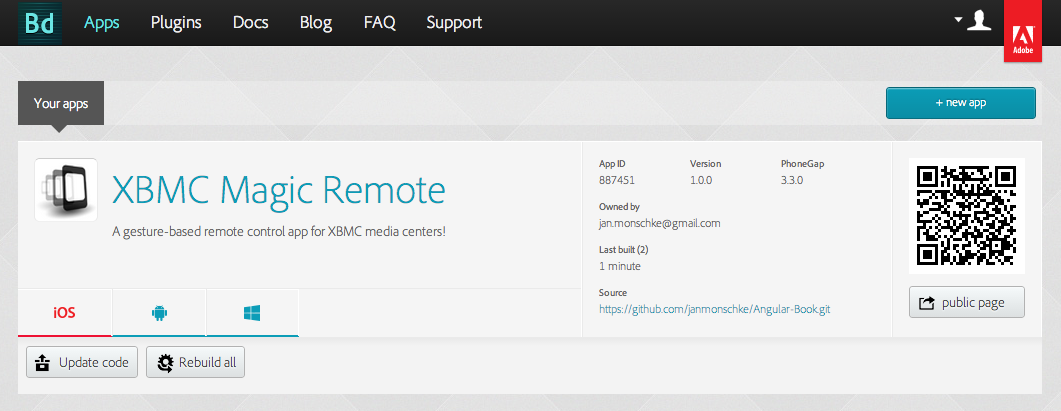
\includegraphics[width=\linewidth]{images/phonegap_build.png}
  }
  \caption[Phonegap Build]{Phonegap Build}
  \label{fig:phonegap-build}
\end{figure}

In addition to providing just the build chain for packaging apps, the Phonegap project also provides an easy to use web application that automatically creates mobile builds from Github repositories. The builds for XBMCMagic can be found at \url{https://build.phonegap.com/apps/887451/share}.